\section{Creating the Model Data from Raw Data}\label{Sec:Creating the Model Data from Raw Data}

We begin with raw data, $\rho^{\raw}, T^{\raw}, p^{\raw}$, and
$X^{\raw}$.  Here is the raw data file for each test problem:
\begin{eqnarray}
{\tt test2} & \rightarrow & \mathrm{none-it~ is~ generated~ analytically} \nonumber \nonumber \\
{\tt test\_convect} & \rightarrow & \mathrm{none-it~ is~ generated~ analytically} \nonumber \nonumber \\
{\tt wdconvect} & \rightarrow & {\tt initial\_models/kepler/model\_6.e8.raw} \nonumber \\
{\tt spherical\_heat} & \rightarrow & \mathrm{none-it~ is~ generated~ analytically} \nonumber \\
{\tt xrb} & \rightarrow & {\tt initial\_models/xrb/sorted\_xrb.raw} \nonumber
\end{eqnarray}
Using the raw data, we need to generate model data with the same
resolution as the base state.  Note that for spherical problems we set
$\Delta r = \Delta x/\mathtt{drdxfac}$.  We use a fortran subroutine
to interpolate the raw data, yielding the model data, $\rho^{\model},
T^{\model}, p^{\model}$, and $X^{\model}$.  The fortran subroutine
then uses an iterative procedure to modify the model data so that it
is thermodynamically consistent with the {\tt MAESTRO} equation of
state (EOS), and also satisfies our chosen hydrostatic equilibrium
(HSE) discretization,
\begin{equation}
\frac{p_r - p_{r-1}}{\Delta r} = \frac{\rho_r + \rho_{r-1}}{2}g,\label{HSE Discretization}
\end{equation}
to a user defined tolerance.  Here are the fortran subroutines for each test problem:
\begin{eqnarray}
{\tt test2} & \rightarrow & {\tt initial\_models/test2/init\_1d.f90} \nonumber \\
{\tt test\_convect} & \rightarrow & {\tt initial\_models/test2/init\_1d.f90} \nonumber \\
{\tt wdconvect} & \rightarrow & {\tt initial\_models/kepler/init\_1d.f90} \nonumber \\
{\tt spherical\_heat} & \rightarrow & {\tt initial\_models/spherical/init\_1d.f90} \nonumber \\
{\tt xrb} & \rightarrow & {\tt initial\_models/xrb/init\_1d.f90} \nonumber
\end{eqnarray}
The model data is not generated at run-time - it must be generated in
advance of running any MAESTRO examples.  The inputs file should point
to the file containing the model data.

\subsection{Multilevel Plane-Parallel}
We do the same thing as the single-level case except that we generate
model data with the same resolution as the finest base state
resolution.


\section{Creating the Initial Data from the Model Data}
In {\tt base\_state.f90}, using the subroutine {\tt
  init\_base\_state.f90} (which is actually a terrible name since we
are setting the initial data, not the base state), we set the initial
data $\rho^{\init}, T^{\init}, p^{\init}$ and $X^{\init}$ equal to the
model data.  Then, we set $h^{\init} =
h^{\init}(\rho^{\init},T^{\init},X^{\init})$.  Note that in the code,
$p^{\init}$ is also overwritten, but the value of $p^{\init}$ does not
change since we called $p^{\model} =
p^{\model}(\rho^{\model},T^{\model},X^{\model})$ at the end of the
fortran subroutine in \S~\ref{Sec:Creating the Model Data from Raw
  Data}.

\subsection{Multilevel Plane-Parallel}
We do the same thing as the single-level case except that we generate
initial data at the non-finest levels by using linear interpolation
from the two nearest model points (see Figure \ref{Fig:Multilevel
  Initialization}).  Note that the initial data is not in HSE nor is
it thermodynamically consistent on non-finest cells.  We will enforce
these on the base state and full state later.
%%%%%%%%%%%%%%%%%%%%%%%%%%%%%%%%%
\begin{figure}[tpb]
\centering
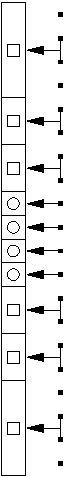
\includegraphics[width=0.4in]{\figpath/multilevel_init}\hspace{0.2in}
\begin{minipage}[b]{5.0in}
\caption{Multilevel Initialization.  The data from the initial model
  is represented by the dots on the right.  The initial data at the
  finest level is represented by the circles.  The initial data at
  non-finest levels is represented by the squares.  We copy data from
  the dots directly into the circles.  We use linear interpolation
  using the two nearest points to copy data from the dots to the
  squares.\vspace{2em}}
\end{minipage}
\label{Fig:Multilevel Initialization}
\end{figure}
%%%%%%%%%%%%%%%%%%%%%%%%%%%%%%%%%


\section{Creating the Base State and Full State}\label{Sec:Creating the Base State and Full State}

Given $p^{\init}, \rho^{\init}, T^{\init},$ and $X^{\init}$, this
section describes how the base state ($\rho_0$ and $p_0$) and full
state ($\rho, h, X$, and $T$) are computed.  We require that $\rho_0 =
\overline\rho$, the base state is in HSE according to equation
(\ref{HSE Discretization}), and the full state is thermodynamically
consistent with $p_0$.  Here are the steps:
\begin{enumerate}
\item Fill $\rho^{\init}, h^{\init}, X^{\init}$, and $T^{\init}$ onto a 
  multifab to obtain the full state $\rho, h, X$, and $T$.
\item If {\tt perturb\_model} = F, skip the remaining steps and
  instead set $p_0 = p^{\init}$ and $\rho_0 = \rho^{\init}$.
\item Perturb $T$, then compute $\rho,h = \rho,h(p^{\init},T,X)$.
\item Set $\rho_0 = \overline\rho$.
\item Compute $p_0$ using equation (\ref{HSE Discretization}), using
  the $p^{\init}$ at the top of the domain as the one required boundary 
  condition.  Note that we still integrate upwards from the bottom, but then
  offset the final pressure so the pressure at the top of the domain
  remains unchanged.
\item Compute the full state $T,h = T,h(\rho,p_0,X)$.
\item Set $(\rho h)_0 = \overline{(\rho h)}$.
\end{enumerate}
Now $\rho_0 = \overline\rho$, the base state is in HSE, and the full
state is thermodynamically consistent with $p_0$.

\subsection{Multilevel Plane-Parallel}
\begin{enumerate}
\item Fill $\rho^{\init}, h^{\init}, X^{\init}$, and $T^{\init}$ onto
  a multifab to obtain the full state $\rho, h, X$, and $T$.
\item If {\tt perturb\_model} = F, skip the next two steps and instead
  set $\rho_0 = \rho^{\init}$.
\item Perturb $T$, then compute $\rho,h = \rho,h(p^{\init},T,X)$.
\item Set $\rho_0 = \overline\rho$.
\item Compute $p_0$ using equation (\ref{HSE Discretization}), using
  the pressure at the top of the domain as the initial condition.
  Note that we still integrate upwards from the bottom, but then
  offset the final pressure so the pressure at the top of the domain
  remains unchanged.  Use the coarse-fine interface discretizations
  given in \S~\ref{Sec:Coarse-Fine HSE Discretization}.
\item Compute the full state $T,h = T,h(\rho,p_0,X)$.
\item Set $(\rho h)_0 = \overline{(\rho h)}$.
\end{enumerate}
Now $\rho_0 = \overline\rho$, the base state is in HSE, and the full
state is thermodynamically consistent with $p_0$.

\subsection{Coarse-Fine HSE Discretization}\label{Sec:Coarse-Fine HSE Discretization}
Integrating the HSE discretization upward, when we encounter a change
from coarse to fine, here is an equation to integrate up to the
coarse-fine interface ($l$ is the ``finer'' level, $l-1$ is the
``coarser'' level)
\begin{equation}
\frac{p_{r-\myhalf}^l - p_{\sfrac{r}{2}-1}^{l-1}}{\Delta r^{l-1}/2} = \frac{\rho_{r-\myhalf}^l + \rho_{\sfrac{r}{2}-1}^{l-1}}{2}g ~~~ \rightarrow ~~~ p_{r-\myhalf}^l = p_{\sfrac{r}{2}-1}^{l-1} + \frac{\Delta r^{l-1} g}{4}\left(\rho_{r-\myhalf}^l + \rho_{\sfrac{r}{2}-1}^{l-1}\right).
\end{equation}
Here is an equation to integrate from the coarse-fine interface up to
the cell center
\begin{equation}
\frac{p_r^l - p_{r-\myhalf}^l}{\Delta r^l/2} = \frac{\rho_r^l + \rho_{r-\myhalf}^l}{2}g ~~~ \rightarrow ~~~ p_r^l = p_{r-\myhalf}^l + \frac{\Delta r^l g}{4}\left(\rho_r^l + \rho_{r-\myhalf}^l\right).
\end{equation}
Combining equations gives
\begin{equation}
p_r^l = p_{\sfrac{r}{2}-1}^{l-1} + \frac{\Delta r^{l-1} g}{4}\left(\rho_{r-\myhalf}^l + \rho_{\sfrac{r}{2}-1}^{l-1}\right) + \frac{\Delta r^l g}{4}\left(\rho_r^l + \rho_{r-\myhalf}^l\right).
\end{equation}
We can simplify using
\begin{equation}
\Delta r^{l-1} = 2\Delta r^l,
\end{equation}
\begin{equation}
\rho_{r-\myhalf}^l = \frac{2}{3}\rho_r^l + \frac{1}{3}\rho_{\sfrac{r}{2}-1}^{l-1}.
\end{equation}
Simplifying
\begin{eqnarray}
p_r^l &=& p_{\sfrac{r}{2}-1}^{l-1} + \frac{\Delta r^l g}{2}\left(\frac{2}{3}\rho_r^l + \frac{1}{3}\rho_{\sfrac{r}{2}-1}^{l-1} + \rho_{\sfrac{r}{2}-1}^{l-1}\right) + \frac{\Delta r^l g}{4}\left(\rho_r^l + \frac{2}{3}\rho_r^l + \frac{1}{3}\rho_{\sfrac{r}{2}-1}^{l-1}\right) \nonumber \\
&=& p_{\sfrac{r}{2}-1}^{l-1} + \frac{3\Delta r^l g}{4}\left(\rho_{\sfrac{r}{2}-1}^{l-1} + \rho_r^l\right).\label{Coarse-Fine Stencil}
\end{eqnarray}
When we encounter a change from fine to coarse, analogously
\begin{equation}
p_{(r+1)/2}^{l-1} = p_{r}^l + \frac{3\Delta r^l g}{4}\left(\rho_{r}^l+\rho_{(r+1)/2}^{l-1}\right).\label{Fine-Coarse Stencil}
\end{equation}

